Validation of Napali hinges on the validation of performance of the OPQ Boxes. Some of the detection capability of the OPQ Boxes has already been characterized as shown in the previous section, however transient response and the $V_{rms}$ response are yet to be confirmed. Once the OPQ Box sensitivity has been characterized, the detection capability of Makai system must be crosschecked. First synthetic triggering streams will be injected into Makai. Next the full system will be deployed at the University of Hawaii Manoa for in-situ validation.

\section{OPQ Box Validation.}
So far only the frequency sensitivity of the OPQ Box has been validated empirically. The transient and as well as $V_{rms}$ response characterization will first be performed using synthetic data. Robust methods for generating power quality events are present in literature, and thus no new research for single device validation is required.\cite{kumar2015power}\cite{tan2013simulation} Next once the DSP software is characterized, synthetic PQ data will be loaded into a SDG1025 signal generator, and fed into the OPQ Box hardware. Any discrepancy between the DSP, and hardware-in-the-loop characterization will be noted and analyzed. The main characteristics to be validated are as follows:
\begin{itemize}
  \item{DC response:} Accuracy of the OPQ Box in measurement of a DC voltage.
  \item{$V_{rms}$ response:} Accuracy of the OPQ Box in measurement of a small changes in the amplitude of AC waveform.
  \item{THD response:} Accuracy of the OPQ Box in measurements of small harmonics mixed with a large fundamental AC waveform.
  \item{Transient response:} Validating the response of the OPQ Box metrics to various transients.
\end{itemize} 
These tests will provide a baseline for the detection capabilities of the Napali system, and result in a publication regarding the OPQ Box detection capabilities.

\section{Napali Validation.}
In order to validate the OPQ system as a whole, it will be deployed across the University of Hawaii Manoa campus (UH). This location is ideal because it is a relatively isolated microgrid connected to the Oahu powergrid only via a single 46kV feeder as shown in Figure \ref{expdes:fig:1}. Another advantage of the UH campus is the high number of smart meters deployed across various levels of the power delivery infrastructure. While these meters are mainly geared towards monitoring power consumption they do have some power quality monitoring capabilities. Data provided from these meters can be used in two distinct applications. First of all, this data can be used to pinpoint the sections of the University of Hawaii power grid which experience a higher likelihood of power quality disturbances. These portions of the grid will have a higher spacial density of OPQ Boxes. Secondly, data from the campus deployed meters can be used as ground truth for comparison against the measurements, and analysis performed by the OPQ project. The location of smart meters in the grid topology is shown in figure \ref{expdes:fig:1} as the $M$ nodes. As evident by the meter location none of them are monitoring the consumer level power and mainly focus on the higher voltage power delivery. This placement is evidenced from the smart meter role as a consumption monitor, and thus the deployment of the OPQ Boxes at the residential level will compliment the current power quality monitoring capabilities without introducing redundancies. Finally, the University of Hawaii power grid is supplying a highly diverse infrastructure. Beyond the traditional residential equipment such as computers and consumer grade electronics, the UH power grid powers scientific and laboratory equipment, machine shops, and server farms. All of these elements have varying requirements/tolerances for power quality anomalies as well as different levels of power quality ``pollution''. Furthermore, some of the electricity consumers in the UH campus are entirely unique. For example, the free electron laser located in the Watanabe Hall is one of the only free electron lasers in the world, and the impact/sensitivity of power quality on the instrument are completely unstudied.
\begin{figure}[h]
	\centering
	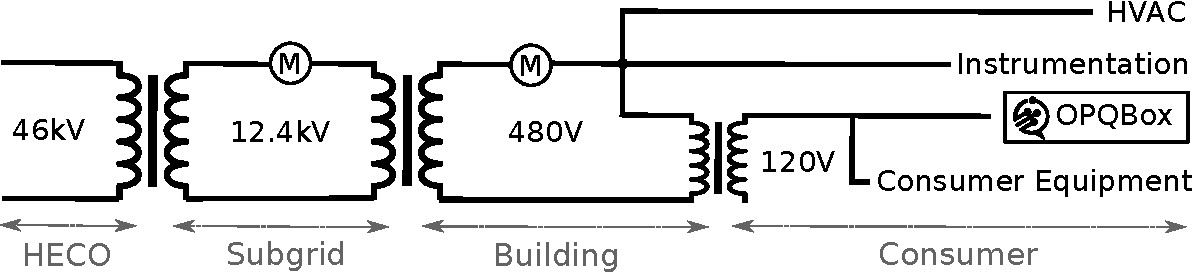
\includegraphics[width=1\linewidth]{img/uh-grid.pdf}	
	\caption{University of Hawaii at Manoa power delivery infrastructure.}
	\label{expdes:fig:1}
\end{figure}

There are 74 smart meters deployed across the UH campus. These meters measure the fundamental frequency $V_{rms}$, power consumption, reactive power, and power factor. Data from these meters will be cross-referenced with the Napali detection system in order to ascertain it's benefits. Validations of the benefits of the Napali framework will follow the framework described in Section \ref{intro:sec:claim}. Here we examine the analysis required to complete each claim in detail.

\subsection{Napali Bandwidth usage} \label{iexp:sec:band}
In order to analytically compute the bandwidth savings of the Napali compared to a system which sends all the data to the sink, I will keep track of the amount of bandwidth the Napali monitoring system consumed during its deployment on UH campus. This will in turn be compared to the bandwidth required by the OPQ Boxes if they were sending the entirety of the data to the sink, and establish the bandwidth efficiency of the Napali framework. In order to monitor the bandwidth of the system in-situ, an iptables bandwidth accounting will be enabled on the sink node. With the accounting enabled, I will be able to extract the exact amount of bytes transfered by the Napali framework during the deployment period. Since the sampling rate of the OPQ Box is well characterized, and the number of OPQ Boxes is fixed, it is trivial to calculate the amount of raw data generated by the OPQ network during any time period. In order to make this comparison fair, the raw data bandwidth will be scaled by the compression ratio of the state of the art compression algorithm specifically designed for power quality measurements.\cite{zhang2009new}

Operating at 12kSps, OPQ Box produces raw data at 24KB/s. With state of the art compression operating at 90\% compression ratio and a 5\% overhead of TCP/IP and meta-data, one can expect a ~3KB/s stream of raw data for each OPQ box if it were to send the entirety of it to the sink. In synthetic experiments, under steady state conditions, OPQ Box consumes 0.5KB/s of bandwidth sending metrics to the Makai. However, this figure does not take into account sending the raw data samples in case an event is detected. The result of bandwidth consumption evaluation will provide a comparison of the bandwidth consumption by Napali methodology of sending metrics and temporal raw data windows of interest compared to sending the entirety of raw data to the sink.

\subsection{Sink processing requirement under the Napali Framework} \label{iexp:sec:scale}
In order to evaluate the scalability of the sink node under the Napali framework, synthetic data containing a small amount of distributed events will be injected into the Makai triggering system. While the synthetic data for a single point PQ disturbance is easily generated, distributed PQ event generation is not well understood. However there is some literature concerning power fault propagation and localization. \cite{parsons1998direction} \cite{polajvzer2017evaluation} The main takeaway from these authors is the energy and amplitude of the event diminishes with electrical distance from the source. As such, by generating a single point PQ event as described in \cite{kumar2015power}\cite{tan2013simulation}, and linearly scaling it based on the simulated electrical distance from the source, a distributed PQ event ensemble can be generated. These events will be ran through the simulated OPQ Box DSP stack and the extracted metrics will be propagated to the Makai aggregation sink. The number of simulated OPQ Box devices that can be supported on a single node will be recorded, and will provide the baseline for the Makai sink node capabilities. Next, the same dataset will be processed on the same node using simulated OPQ Box software stacks. The amount of concurrent processes which are able to keep up with the targeted sampling rate of $12kS/s$ will be determined and recorded, and compared to the amount of devices which can be supported by Makai.

The result of this evaluation will provide a scalability metric for the Napai framework for a single sink node. There are independent metrics which will be presented. First, the number of OPQ Boxes which can reliably send metrics to a single Makai instance for processing will be established. This number is expected to be quite high since the bandwidth and computational requirements for processing the triggering stream are quite low. Second, the number of OPQ Boxes, that can experience and reliably send an event to Makai at the same time will be established. The bandwidth requirement for raw data acquisition is significantly higher then the triggering stream, however there is no computation involved in storing raw data frames. Both of these metrics will be compared to the scalability of performing the entirety of processing on the sink node.

\subsection{Effects of latency in the Napali framework} \label{iexp:sec:lat}
The latency of Napali triggering system has a significant impact on its ability to read out complete raw data events. Using generated distributed events as a baseline, I will be able to tune the threshold and temporal requirements for Makai detection algorithms. Furthermore, temporal, spacial, and amplitude noise will be injected into the generated datasets, to simulate various uncertainties with regards to data collection, such as local noise, and NTP offset errors. Taking into the account the detection latency of Makai, if some of the requested data is no longer available on the OPQ Box, only a partial time window will be returned. These events will be marked as incomplete and their fraction as compared to the total number of events recorded will be used to establish the latency tolerance of the Napali framework. Synthetic benchmarks will be carried out to establish the latency that the Napali system can incur without losing a portion of the event. Since this is highly dependent on the amount of storage allocated for the RDRB, these experiments will be carried out with various RDRB settings.

Because OPQ Boxes operate using public University of Hawaii WIFI, the latency figures for data transmission are expected to be very dynamic. In situations with large network contention, greater then 100ms one way packet latency can be expected. This latency is exacerbated since at least three separate communication steps are required before raw data is received by Makai. First the metric has to be sent to Makai, next if Makai detects an event, a data request needs to be sent to the affected boxes. Finally boxes will forward raw data to the Makai sink. I expect that with RDRB capacity of storing 5 seconds of raw data, no raw data events of 1s or shorter will be missed. This figure allows for 1 second of transfer latency, 3 seconds of Makai analysis latency, and leaves 1 second of data in RDRB for readout. However, these figures can only be validated in a real world situations.

\subsection{Temporal locality triggering of the Napali framework} \label{iexp:sec:loc}
Once the OPQ Box is fully validated and the Makai detection thresholds are tuned using synthetic datasets, the Napali system will be fully deployed at the University of Hawaii at Manoa.  Every time the Napali detects an event, both OPQ Boxes and building meters will be queried for data. While it may be unfeasible to query raw data from the UH metering infrastructure, metrics are readily available. This data will be used to ascertain the proportion of false positive events detected by Napali. Additionally, the internal single point fault detection mechanism of the UH power meters will be used in conjunction with the events detected by Napali to measure the rate of false negative events. Both the false negative and false positive measurements will be used to ascertain the detection efficient of the Napali framework. This analysis will also include an evaluation  of Napali's ability to reject single point anomalies. For a portion of OPQ deployment, every event triggered by a single device will be captured. These events will be analyzed in order to determine if a gridwide anomaly was incorrectly classified as a single point disturbance. 

The goal of Napali is not to to provide a zero false positive rate. Once raw data is stored, higher level processing can further filter and classify it using more computationally expensive techniques. As long as the bandwidth consumption of Napali compares favorably to sending the entirety of raw data to the sink, any rate of false positives can be tolerated. False negatives on the other hand are the primary metric subject to optimization. Ideally a zero rate of false positives would be expected, however as with any real-world system I do not expect that to be the case. This evaluation will determine the triggering efficiency of the Napali framework when compared to the detection ability of a commercially available system.

\subsection{Sub-threshold Data Acquisition} \label{iexp:sec:sub}
The Napali methodology will be compared with the single point anomaly detection approach. In order to do that I will compare the extent to which sub-threshold events are missed by the UH metering infrastructure. In a large distributed event, if a portion of events are not detected by the UH meter's single point detection, but picked up by the Napali framework, these events will be flagged and analyzed for their merit. This will in turn provide a metric of distributed detection ability of the Napali framework compared to commercial system. Furthermore, for a portion of the deployment the triggering stream from the OPQ Boxes will be stored along with the acquired raw data. The triggering stream can be used to compute which fraction of devices would have self triggered if operating autonomously. This will provide the baseline for sub-threshold triggering efficiency of the Napali system, with respect to the single point detection ability of the OPQ Box.

This evaluation will compare Napali performance to the single point detection mechanisms currently in deployment. I expect that Napali will outperform these strategies, and provide a more complete picture of gridwide anomalies as they propagate through the UH power grid. It is possible that no sub-threshold events will be recorded during the UH deployment. UH campus is quite small, perhaps too small for an anomaly in one building not to impact the rest of campus. In this case the sub-threshold data acquisition will remain an open topic for future work and a larger geographical deployment. Regardless, as long as I am be able to validate the single point anomaly rejection ability of Napali as described in Section \ref{iexp:sec:loc}, I will be able to conclude that Napali has a distinct advantage over single point detection methods. Single point anomalies are not important in smart grid monitoring, since they originate from the consumers side of the meter, and should be ignored. In fact, recording these events may be detrimental to the privacy of the end-user, since it may give clues on their activities as shown in Figure \ref{intro:fig:1} a and b. However since privacy implication of power quality monitoring are outside the scope of this project, this study will remain as a point of future work.

\section{Napali Framework in Other Domains}
The work outlined above will allow me to characterize the benefits and drawbacks of the Napali architecture. Armed with this knowledge I intend to examine the examine the possibility of using a similar architecture in other domains. The Napali approach could prove useful in general sensor network design, as well as IOT and other domains which rely on anomaly detection. This contribution will involve an additional literature review of anomaly detection systems, and proposals to integrate Napali-like methodology to improve their efficiency and reduce their bandwidth consumptions. It will also include a discussion of hardware design changes required to existing sensors in these other domains in order to support the Napali framework.


\section{Schedule}
Bellow is the time-line describing the major research activities leading up to my defense.

\begin{center}
\begin{tabular}{ ||c | c c|| }
\hline
 \textbf{Activity} & \textbf{Start Date} & \textbf{End Date} \\ 
 \hline
 \hline
 OPQ Box 2 Validation & October 1\textsuperscript{st} & November 31\textsuperscript{st} \\  
 Makai Validation & October 15 1\textsuperscript{st} & November 30\textsuperscript{th}   \\
 Data Collection & December 1\textsuperscript{st} & TBD   \\
 OPQ Box 2 Instrumentation paper & January 1\textsuperscript{st} & February 1\textsuperscript{st}   \\
 Data Analysis & February 1\textsuperscript{st} & March 1\textsuperscript{st}  \\
 Introduction Dissertation Chapter & March 1\textsuperscript{st}  & March 15\textsuperscript{th}  \\
 Literature Review Dissertation Chapter & March 15\textsuperscript{th} & April 1\textsuperscript{st}  \\
 Experimental Design Dissertation Chapter & April 1\textsuperscript{st} & April 15\textsuperscript{th}  \\
 Analysis Dissertation Chapter & April 15\textsuperscript{th} & May 15\textsuperscript{th}  \\
 Conclusions Dissertation Chapter & May 15\textsuperscript{th} & June 15\textsuperscript{th}  \\
 \hline
 
\end{tabular}
\end{center}
